% globale Parameter (Papierformat, Schriftgroeße, Trennlinien, Doppelseitig)
\documentclass[a4paper, 11pt, headsepline,footsepline,twoside,abstract]{scrbook}


%%% Verwendete Pakete %%%

\usepackage{url}
\usepackage{geometry} % Seitenraender
\usepackage{fancyhdr} % Schoenere Kopf/Fußzeilen
\usepackage[utf8]{inputenc} % Kodierung
\usepackage[ngerman]{babel} % Sprache
\usepackage{graphicx}  % Bildchen
\usepackage{float}  % Bildchen2
\usepackage{setspace} % fuer Zeilenabstand
\usepackage[T1]{fontenc} % fuer Schriftart
%\usepackage{cite} % fuer Zitate
\usepackage[numbers,square]{natbib} % Package für Zitierstil
\usepackage{pgfplots} % Plots
\usepackage[justification=RaggedRight, singlelinecheck=false, margin=1.5cm]{caption}  % huebschere Captions
\usepackage[version=3]{mhchem} % chemische Formeln
\usepackage{booktabs} % schoenere Tabellen
\usepackage{multirow} % s.o.
\usepackage{ifthen} % s.o.
\usepackage{subfigure} % Grafiken nebeneinander darstellen
\usepackage{textcomp} %Euro-Zeichen
\usepackage{siunitx} % Einheiten korrekt anzeigen
%\sisetup{
% locale = DE ,
% per-mode = symbol,
% separate-uncertainty %+- Notation
%}
%\DeclareSIUnit{\masspercent}{m\%}
%\newcommand{\euro}{\,\texteuro\ } %Euro einfuegen

%Schriftart aendern
\newcommand{\changefont}[3]{
\fontfamily{#1} \fontseries{#2} \fontshape{#3} \selectfont}
\changefont{ptm}{m}{n}

% Zeilenabstand 1,5
\onehalfspacing

% weniger breite Seitenraender
\geometry{a4paper,left=28mm,right=28mm, top=32mm, bottom=30mm} 

% Keine Einrueckung bei neuen Absätzen
%\setlength{\parindent}{0pt}
%\setlength{\parskip}{\baselineskip}

% Bissel Tabellenmagie
\newcommand{\forloop}[5][1]{%
\setcounter{#2}{#3}%
\ifthenelse{#4}{#5\addtocounter{#2}{#1}%
\forloop[#1]{#2}{\value{#2}}{#4}{#5}}%
{}}

\newcounter{crcounter}

\newcommand{\compensaterule}[1]{%
\forloop{crcounter}{1}{\value{crcounter} < #1}%
{\vspace*{-\aboverulesep}\vspace*{-\belowrulesep}}}

\newcommand{\multirowbt}[3]{\multirow{#1}{#2}%
{\compensaterule{#1}#3}}

%%% Kopf und Fußzeilendesigns %%%

% normaler Style
\fancypagestyle{normal}
{
\fancyhead[EL]{\thepage}
\fancyhead[ER]{\leftmark}
\fancyhead[OL] {\rightmark}
\fancyhead[OR]{\thepage}
\fancyfoot[OL]{\parbox[b][0.04\columnwidth][t]{0.5\textwidth}{\raggedright Masterarbeit, Christoph Gielisch}}
\fancyfoot[OR]{
	
\includegraphics[height=0.05\columnwidth]{images/IAM_Logo.png}
	%\caption{}
	\label{img:grafik-dummy}
	}
\fancyfoot[OC,EC]{}
\fancyfoot[EL]{
	
\includegraphics[height=0.05\columnwidth]{images/KIT_LOGO.png}
	%\caption{}
	\label{img:grafik-dummy}
	}
\fancyfoot[ER]{\parbox[b][0.04\columnwidth][t]{0.5\textwidth}{\raggedleft  Thema Masterarbeit}}
\renewcommand{\headrulewidth}{0.5pt}
\renewcommand{\footrulewidth}{0.5pt}
}

% Kapitelanfaenge bekommen ein extra Kopf/Fußzeilendesign
\fancypagestyle{plain}
{
\fancyhf{} % clear all header and footer fields
\fancyfoot[R]{\parbox[b][0.04\columnwidth][t]{0.5\textwidth}{\raggedleft \thepage}}
\fancyfoot[L]{
	
\includegraphics[height=0.05\columnwidth]{images/leerpixel.png}
	%\caption{}
	\label{img:grafik-dummy}
	}
\renewcommand{\headrulewidth}{0pt}
\renewcommand{\footrulewidth}{0.5pt}
}

% Die Inhaltsangabe auch
\fancypagestyle{toc}
{
\fancyhf{} % clear all header and footer fields
\fancyfoot[OR]{\parbox[b][0.04\columnwidth][t]{0.5\textwidth}{\raggedleft \thepage}}
\fancyfoot[OL]{
	
\includegraphics[height=0.05\columnwidth]{images/leerpixel.png}
	%\caption{}
	\label{img:grafik-dummy}
	}
\fancyfoot[EL]{\parbox[b][0.04\columnwidth][t]{0.5\textwidth}{\raggedright \thepage}}
\fancyfoot[ER]{
	
\includegraphics[height=0.05\columnwidth]{images/leerpixel.png}
	%\caption{}
	\label{img:grafik-dummy}
	}
\renewcommand{\headrulewidth}{0pt}
\renewcommand{\footrulewidth}{0.5pt}
}

% Festlegung Art der Zitierung
%\bibliographystyle{unsrtdin}

%%%%%%%%%%%%%%%%%%% hier beginnt das Dokument %%%%%%%%%%%%%%%%%%%%
\begin{document}

\thispagestyle{empty}
\begin{center}
%\Large{Karlsruher Institut für Technologie}\\
\end{center}

\begin{figure}
	\centering
	
\includegraphics[width=0.5\columnwidth]{images/KIT_LOGO.png}
	%\caption{}
	\label{img:grafik-dummy}
\end{figure}

\begin{center}
\textbf{\huge{ Aufbau einer in-situ Li$^7$-NMR\\[0.4cm]Batterietestzelle}}
\end{center}
\begin{center}
\large{}
\end{center}
\begin{center}
\textbf{\Large{}}
\end{center}
\begin{center}
\large{Von der Fakultät für Wirtschaftswissenschaften des \\ Karlsruher Instituts für Technologie genehmigte }
\end{center}
\begin{verbatim}

\end{verbatim}
\begin{center}
\textbf{\LARGE{Masterarbeit}}
\end{center}
\begin{center}
am
\end{center}
\begin{center}
\textbf{\Large{Institut für Angewandte Materialien - Keramische Werkstoffe und Technologien (IAM-KWT)}}
\end{center}
\begin{center}
von
\end{center}
\begin{center}
\Large{Christoph Gielisch}
\end{center}
\begin{verbatim}

\end{verbatim}
\begin{center}
30. September 2015
\end{center}
\begin{verbatim}

\end{verbatim}
\begin{center}
\textbf{Referent:} \\ Prof. Dr-Ing. Volker Schulze \\
\textbf{Koreferent:} \\ Prof. Dr. Michael J. Hoffmann\\
\textbf{Betreuer:} \\ Dr. Claudia Bucharsky \\ 
Dr.-Ing. Günter Schell \\
\end{center}
\newpage
\cleardoubleemptypage
% Eidesstattliche Erklärung
\setcounter{page}{1}
\pagenumbering{Roman}
\textbf{\Large{Eidesstattliche Erklärung}}
\\\\
Hiermit erkläre ich, diese Arbeit selbstständig und ohne fremde Hilfe verfasst zu haben. Es wurden nur die in der Arbeit ausdrücklich benannten Quellen und Hilfsmittel benutzt. Wörtlich oder sinngemäß übernommenes Gedankengut ist als solches gekennzeichnet.
\\\\
Karlsruhe, den 30.09.2015
\\\\
\\\\
\\
(Christoph Gielisch) 
 
\newpage

% Eidesstattliche Erklärung2
\setcounter{page}{1}
\pagenumbering{Roman}
\textbf{\Large{Zusammenfassung}}
\\\\
TBD
% Inhaltsverzeichnis
%\KOMAoption{open}{left} 
\pagestyle{toc}
\renewcommand*{\chapterpagestyle}{toc} % Die erste Seite des TOC ist auch ein Kapitelanfang
\tableofcontents
\KOMAoption{open}{right} 
\newpage
\cleardoubleemptypage
\pagestyle{normal}
\renewcommand*{\chapterpagestyle}{plain}
\setcounter{page}{1}
\pagenumbering{arabic}
\chapter{Einleitung}
Batterien nehmen in unserem Leben einen immer höheren Stellenwert ein. Sie kommen in nahezu allen mobilen elektrischen Geräten zum Einsatz. Die im Zuge des Klimaschutzes zunehmende Dekarboniserung von Wirtschaft und Gesellschaft erfordert außerdem, dass bisher mittels fossiler Brennstoffe betriebene Geräte und Maschinen in Zukunft elektrisch betrieben werden. Ein Beispiel ist hier die großflächige Einführung von Elektroautomobilen. Aber auch zur Speicherung von volatil erzeugter Energie, beispielsweise bei Wind- und Sonnenenergie, sind leistungsfähige Batterien nötig.
\\\\
Die vorliegende Arbeit betrachtet die Einsatzmöglichkeit von speziellen Keramiken als Festkörperelektrolyt in Batterien.
\section{Motivation}
Ein Batterie mit einem Festkörperelektrolyten bietet gleich mehrere Vorteile gegenüber der herkömmlichen Flüssigelektrolyt-Batterie. Der Flüssigelektrolyt moderner Lithiumbatterien besteht zumeist aus einem organischem Lösungsmittel und darin gelösten Lithiumsalzen (QUELLE). Diese sind jedoch nicht stabil gegenüber der Luftfeuchtigkeit und reagieren unter der Bildung von ätzenden Substanzen wie Flusssäure ab. Dies ist neben der Unsicherheit beim Versagen der Batterie ebenso auch ein Problem bei der industriellen Großproduktion. Diese kann nur mit großen Anlagen zur Trocknung der Luft erfolgen. Ein Festkörperelektrolyt könnte so gestaltet werden, dass dieser stabil gegenüber der Luftfeuchtigkeit und dem Sauerstoff der Luft ist.
\\\\
Ein weiteres Problem der aktuellen Flüssigelektrolyten ist deren beschränkte Stabilität gegenüber elektrischen Spannungen. Handelsübliche Flüssigelektrolyte sind lediglich bis zu einer Spannung von 4,2V stabil (QUELLE). Es existieren jedoch Hochvoltelektroden, die von höheren Spannungen profitieren würden. Festkörperelektrolyte könnten diesen Mangel beheben.
\section{Zielsetzung}
%Ggf Anpassen
Ziel der vorliegenden Arbeit ist es, verschiedene Keramiken für den Einsatz als Festkörperelektrolyt anzupassen und zu analysieren. Als Ausgangspunkt dienen hierbei die Materialien \ce{LiLaTiO3} (LLTO) sowie \ce{Li_(_1_+_x_)Al_xTi_(_2_-_x_)(PO4)3} (LATP), die in der Literatur bereits eine ausreichend gute Lithiumleitfähigkeit nachweisen konnten (QUELLE). Die Keramiken sollen dabei in Pulverform, als Folienguss, als Tablette und im Gefüge Elektrode-Elektrolyt hergestellt werden. Als Referenz werden auch Elektroden für den Einsatz in normalen Flüssigelektrolyt-Batterien hergestellt und untersucht. Die Festkörperelektrolyte sollen mittels Röntendiffraktometrie (XRD), Kernspinspektroskopie (NMR) und Impedanzspektroskopie untersucht werden. Für die Messung von in-situ-NMR-Daten muss sowohl der Lithium-Probenkopf des NMR-Spektrometers angepasst, als auch eine eigene Testzelle konstruiert und gebaut werden.
\section{Aufbau der Arbeit}
Im ersten Kapitel wird die Arbeit motiviert sowie eine Zielsetzung formuliert. Anschließend werden die nötigen Grundlagen für die durchzuführenden Experimente beschrieben. Das dritte Kapitel beschreibt die Art und Weise der Experimente und deren Durchführung. Die erzielten Ergebnisse werden im vierten Kapitel dargestellt und im fünften Kapitel diskutiert. Das sechste Kapitel bietet eine kurze Zusammenfassung sowie einen Ausblick in die Zukunft.
\chapter{Grundlagen}
Im folgenden Kapitel werden die Grundlagen für die im Rahmen der Arbeit stattgefundenen Experimente gelegt. Dafür wird im ersten Teil der Aufbau und die Elektrochemie sowie die Materialauswahl von Batteriezellen beschrieben. Anschließend werden drei verschiedene Analysemethoden für Festkörperelektrolyte vorgestellt.
\section{Batteriezellen}
\begin{figure}
	\centering
	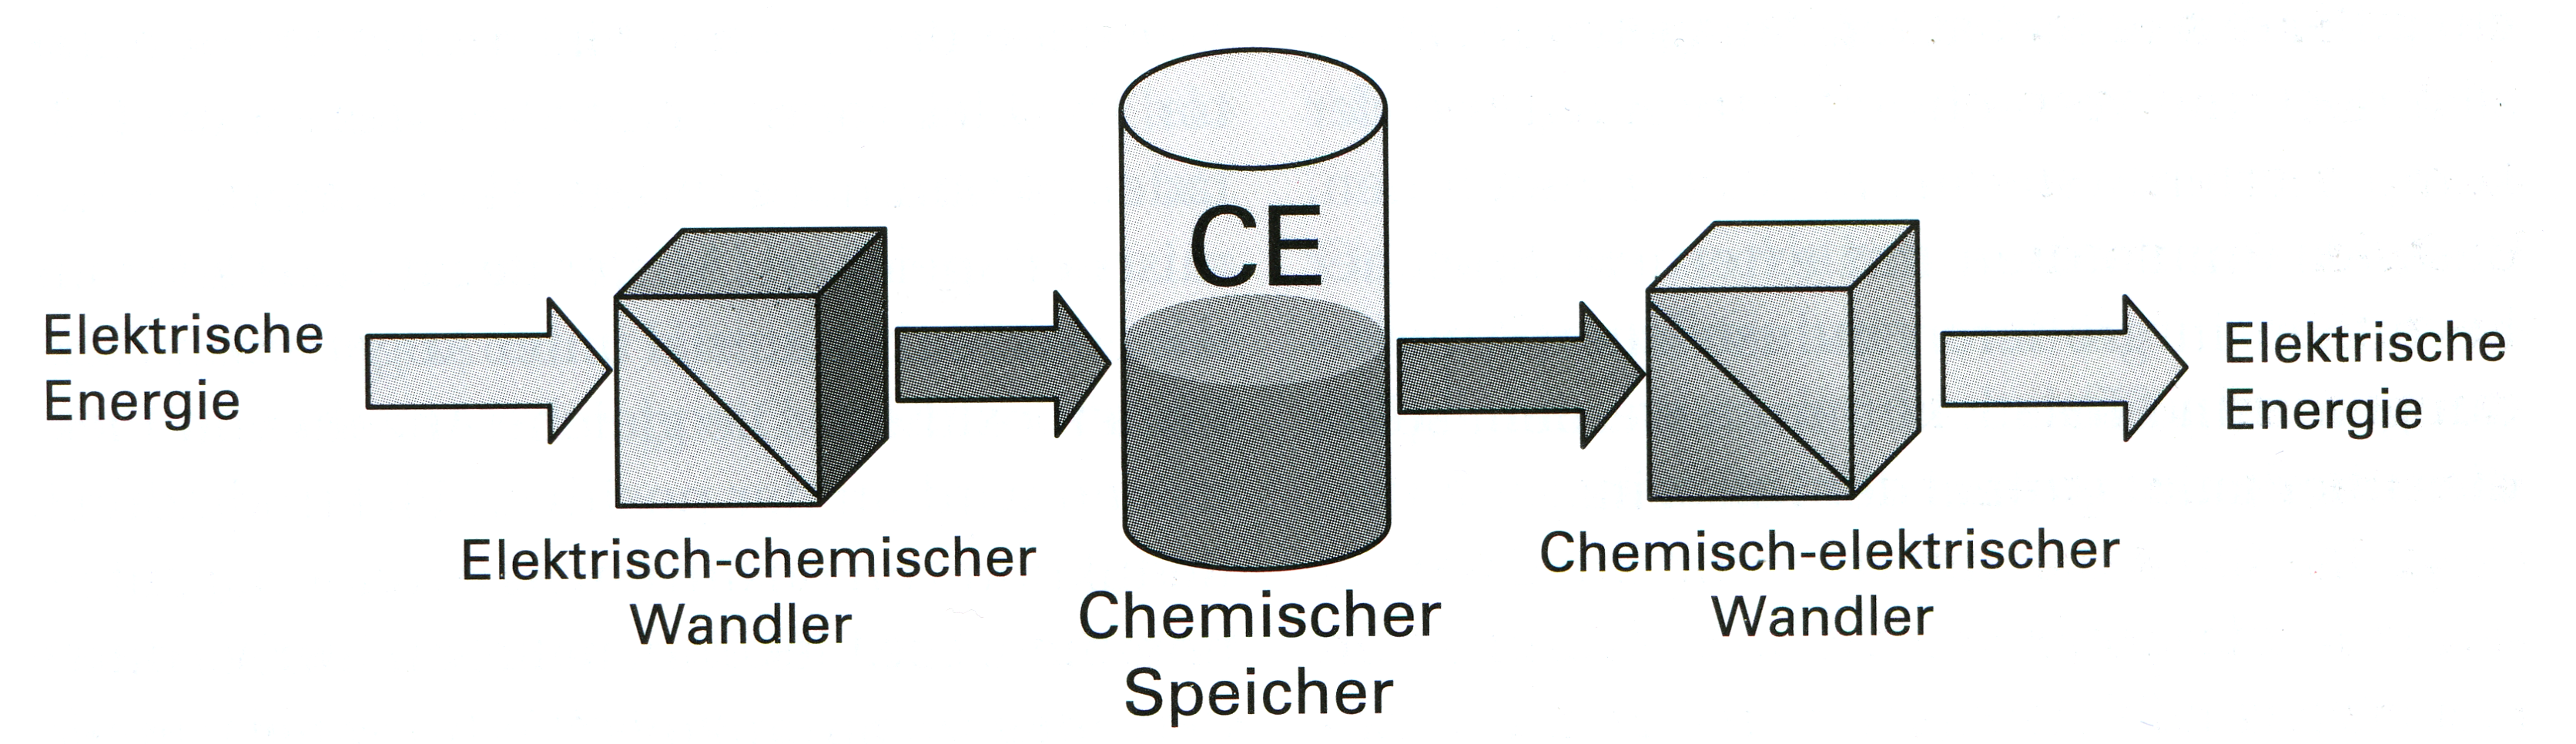
\includegraphics[width=1.0\columnwidth]{images/Prinzipieller_Aufbau.png}
	\caption{Prinzip einer sekundären Zelle}
	\label{Prinzip_Zelle}
\end{figure}
Die Batteriezelle ist eine Form der Galvanischen Zelle. Es lassen sich dabei grundsätzlich drei verschiedene Arten von Galvanischen Zellen unterscheiden:
\begin{description}
\item[Primäre Zelle - Batterie] Primäre Zellen besitzen ein chemisches Potential, welches durch den Anschluss eines externen Verbrauchers als elektrischer Strom abgerufen werden kann. Dieser Vorgang ist jedoch nicht reversibel.
\item[Sekundäre Zelle - Akkumulator] Im Gegensatz zur primären Zelle kann die sekundäre Zelle Energie nicht nur abgeben, sondern auch wieder aufnehmen und speichern. Dieses Verhalten wird in Abbildung \ref{Prinzip_Zelle} dargestellt.
\item[Tertiäre Zelle - Brennstoffzelle] Die Tertiäre Zelle wird kontinuierlich mit einem Brenngas durchflossen und kann daher auch dauerhaft Energie in Form von elektrischen Strom abgeben.  
\end{description}
Die Bezeichnung Akkumulator ist dabei gerade im englischen Sprachgebrauch nicht geläufig, man spricht eher von \textit{rechargeable batteries}, also wiederaufladbaren Batterien. Auch im deutschen geht man dazu über den Begriff Batterie sowohl für primäre als auch für sekundäre Zellen zu gebrauchen. Iim Rahmen dieser Arbeit wird das Wort \textit{Batterie} synonym für beide Arten von Zelle verwendet. Betrachtet werden jedoch nur wiederaufladbare Batterien.
\subsection{Elektrochemischer Vorgang}
\begin{figure}
	\centering
	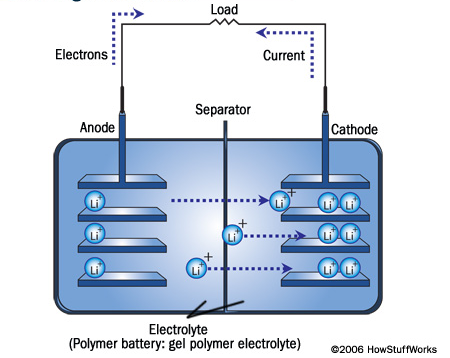
\includegraphics[width=0.6\columnwidth]{images/Schematischer_Aufbau_Li_Ionen.png}
	\caption{Schematischer Aufbau einer Lithium-Ionen-Batterie}
	\label{schema_li_ionen}
\end{figure}
Die Elektrochemie einer Batteriezelle basiert auf einem Potential zwischen zwei räumlich getrennten Materialien. Durch den Anschluss eines externen Stromkreises kann dieses Potential entweder unter Abgabe von Energie abgebaut oder unter Zugabe von Energie vergrößert werden. 
\\\\
Es existieren zwei grundsätzliche Mechanismen zur Ladungsübertragung und Speicherung:
\\\\
\textbf{i) Interkalation}
\\\\
Bei der Interkalation handelt es sich um den reinen Einbau eines Atoms oder Ions in ein Wirtsgitter hinein, ohne das Stattfinden einer Reaktion. Beispiel wäre hier der Einbau von Lithiumkationen in eine Graphitstruktur.
\\\\
\textbf{ii) Redoxreaktion}
\\\\
Während der Redoxreaktion kommt es zu einem Austausch von Elektronen zwischen verschiedenen Edukten. Der reduzierte, also elektronenabgebende, und der oxidierte, also elektronenaufnehmende, Part können dabei räumlich getrennt in den jeweiligen Elektroden vorliegen.
\\\\
Bei einer Interkalation kommt es nicht zum Übertrag von Elektronen (?).
\subsubsection{Bestimmung der Potentialdifferenz}
Das Potential zwischen zwei Materialien kann als Differenz ihrer jeweiligen Nernstschen Halbzellenpotentiale bestimmt werden. Die Nernst-Gleichung definiert:
\begin{equation}
E = E_0 + \frac{RT}{z_eF}\; ln \frac{a_{Ox}}{a_{Red}}
\end{equation}
mit:
\begin{description}\itemsep0pt
\item[E] Elektrodenpotential
\item[E$_0$] Standardelektrodenpotential
\item[R] Gaskonstante
\item[T] absolute Temperatur
\item[z$_e$] Anzahl der übertragenen Elektronen
\item[F] Faraday-Konstante
\item[a] Aktivität des betreffenden Redox-Partners
\end{description}
Einsetzen der Naturkonstanten ergibt als vereinfachte Formel unter der Bedingung eines Betriebes bei Raumtemperatur:
\begin{equation}
E = E_0 + \frac{0,059 V}{z_e} \; log \frac{a_{Ox}}{a_{Red}}
\end{equation}
Die Leerlaufspannung einer Vollzelle ergibt sich dann aus der Differenz zwischen Kathode und Anode:
\begin{equation}
U_{Zelle} = U_{Kathode} - U_{Anode}
\end{equation}
% Hier Formel einfügen
\subsection{Aufbau}
Eine Batterie besteht aus zwei räumlich voneinander getrennten Elektroden. Dabei wird die Elektrode mit dem niedrigeren Halbzellenpotential als Anode, die Elektrode mit dem höheren Halbzellenpotential als Kathode bezeichnet. Zwischen den beiden Elektroden existiert ein Elektrolyt. Dieser ermöglicht den Ladungsaustausch beider Elektroden über den Transfer von Ionen. Um einen Kurzschluss, also einen direkten Ladungsaustausch zwischen beiden Elektroden, zu vermeiden, kann es außerdem nötig sein, einen Separator zwischen beiden Elektroden einzusetzen. Die beiden Elektroden sind jeweils auf einem Stromkollektor aufgebracht, welcher die Kontaktierung der Elektrode nach außen hin ermöglicht.
\\\\
Es gibt verschiedene Bauformen für Batteriezellen.
\begin{figure}
	\centering
	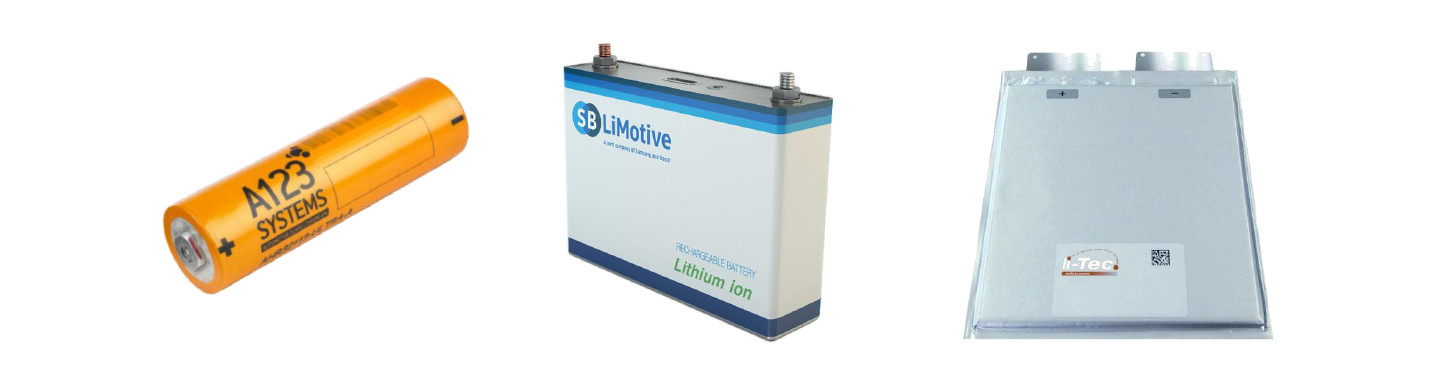
\includegraphics[width=1.0\columnwidth]{images/rund_prisma_pouch.jpg}
	\caption{Vergleich möglicher Bauformen: Rundzelle, prismatische Zelle, Pouch-Zelle}
	\label{vergleich_zellform}
\end{figure}
\begin{description}
\item[Rundzellen] Bei der Rundzellen werden die Stromkollektoren jeweils doppelseitig mit einem Elektrodenmaterial beschichtet und dann abwechselnd aufeinander gestapelt. Anschließend wird die Batteriezelle zu einem Zylinder aufgewickelt.
\item[Prismatische Zellen] Die prismatische Zelle ähnelt im Aufbau der Rundzelle, wird jedoch rechteckig gewickelt und ist so besser schichtbar.
\item[Pouch-Zellen] In diesen Zellen werden meist nur wenige Schichten von Elektroden übereinander gewickelt und anschließend in einer dünnen Hülle gasdicht verschweißt. Ein vor dem Einschweißen durchgeführtes Anbringen eines Vakuums garantiert das Entfernen überflüssiger Gase innerhalb der Zelle.
\item[Knopfzellen] In einer Knopfzelle werden die Elektroden, Elektrolyt und Separator jeweils rund geformt auf einem Boden gestapelt und anschließend mit einem Deckel verschlossen. Eine zusätzlich eingebrachte Feder zwischen Zelle und Deckel sorgt für den notwendigen Anpressdruck, um eine gute Kontaktierung zu gewährleisten.
\end{description}
Eine Übersicht über die verschiedenen Bauformen wird in Abbildung \ref{vergleich_zellform} gezeigt. Batteriezellen können zu Batteriemodulen zusammengeschlossen werden, die dann über ein externes Batteriemanagement gezielt angesprochen und kontrolliert werden können. Ein solcher Aufbau ist in Abbildung \ref{battery_pack} zu sehen.
\\\\
Am IAM-KWT kommen spezielle Testzellen zum Einsatz, deren Aufbau dem von Knopfzellen ähnelt. Die beiden Elektroden und der Elektrolyt werden in eine Glasröhre übereinander montiert. Die Röhre ist über zwei Stopfen mit Dichtungsringen nach außen hin abgedichtet. Eine Druckfeder sorgt für den nötigen Anpressdruck, zwei Edelstahlplättchen für eine homogene Kraftverteilung und Kontaktierung. Verschlossen wird die Zelle mittels Plastikverschlüssen, welche die Stopfen am Verrutschen hindern. Über einfache 2mm-Bohrungen in den Stopfen kann die Zelle mit Bananensteckern an Geräte angeschlossen werden. Die Abbildung \ref{schema_zelle} zeigt die Testzelle schematisch.
\begin{figure}
	\centering
	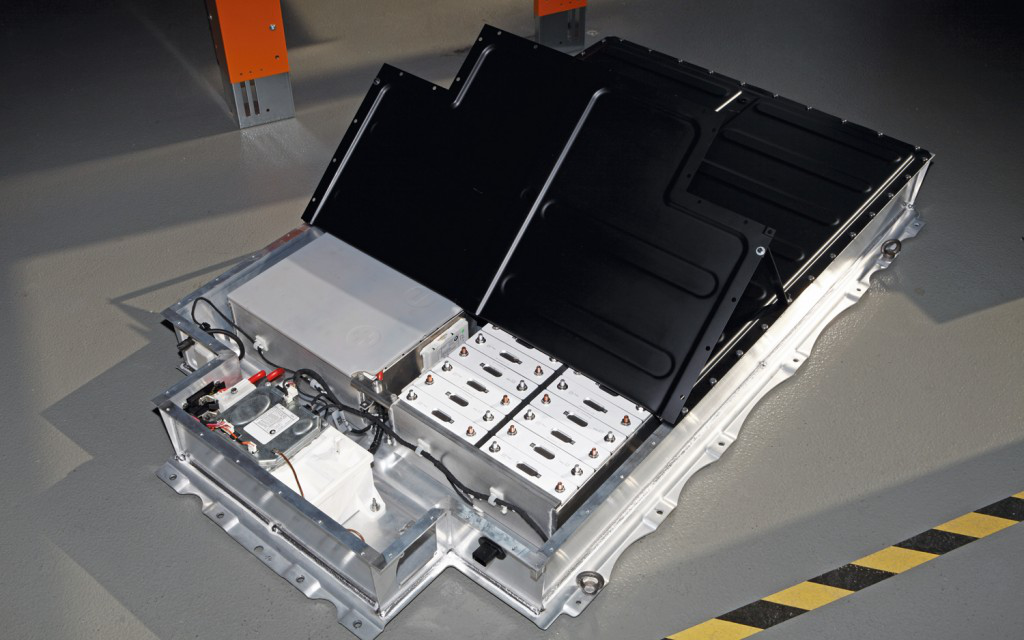
\includegraphics[width=0.9\columnwidth]{images/bmw-i3-battery-pack.png}
	\caption{Battery-Pack des BMW i3 bestehend aus zwei Batteriemodulen und einem Batteriemanagement}
	\label{battery_pack}
\end{figure}
\begin{figure}
	\centering
	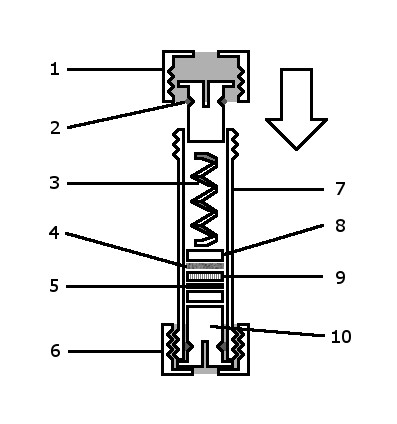
\includegraphics[width=0.7\columnwidth]{images/Schema_Zelle.jpg}
	\caption{Schema der Testzelle; 
			1: Plastikkappe,
			2: Dichtungsring,
			3: Edelstahlfeder,
			4: Kathode,
			5: Anode,
			6: Plastikkappe,
			7: Glaszylinder,
			8: Kontaktierplättchen,
			9: Separator,
			10: Edelstahlstopfen.
			}
	\label{schema_zelle}
\end{figure}
\subsection{Elektrodenmaterialien}
Materialien müssen verschiedene chemische und physikalische Eigenschaften erfüllen, um für den Einsatz in Elektroden geeignet zu sein. Die Ein- oder Auslagerung von Lithium sollte nicht zu einer zu hohen Veränderung des Volumens führen.
\\\\
Die Materialien für Elektroden können grundsätzlich nach ihrem Diffusionsverhalten klassifiziert werden.
\begin{description}
\item[Olivinstruktur] Die Olivinstruktur ist eine eindimensionale Tunnelstruktur, an der entlang die Diffusion stattfindet.
\item[Lagenstruktur] Materialien, die zweidimensionale Diffusion zwischen Schichten ermöglichen, besitzen eine Lagenstruktur.
\item[Spinellstruktur] In der Spinellstruktur ist eine Diffusion in alle drei Richtungen des Raums möglich.
\end{description}
\subsubsection{Typische Anodenmaterialien}
\subsubsection{Typische Kathodenmaterialien}
\section{Keramiken}
\subsection{Perowskite}
\ce{ABO_3}
\subsection{NASICON}
\textbf{Na}-\textbf{S}uper-\textbf{I}onic-\textbf{Con}ductor
\section{Analysemethoden}
Zur Strukturaufklärung werden die Materialien mit unterschiedlichen Analysemethoden untersucht.
\subsection{Röntgendiffraktion}
\subsection{Impedanzspektroskopie}
\subsection{NMR-Spektroskopie}
Die Grundlage der Kernspinresonanzspektroskopie (nuclear magnetic resonance spectroscopy, NMR-Spektroskopie) wurde zum Jahreswechsel 1945/1946 von zwei amerikanischen Forschungsgruppen unabhängig voneinander entwickelt. Felix Bloch und Edward M. Purcell wurden dafür 1952 mit dem Nobelpreis in Physik ausgezeichnet.
\subsubsection{Physikalische Grundlagen der NMR-Spektroskopie}
Die NMR-Spektroskopie nutzt die magnetischen Eigenschaften von Atomkernen und ihren Umgebungen aus, um Aussagen über Zusammensetzungen und Bindungen von Stoffen treffen zu können.
\\\\
Elektronen, Neutronen und Protonen besitzen eine Eigenrotation, den Spin s. Der Spin eines Atomkerns setzt sich aus den Spins der einzelnen Protonen und Neutronen innerhalb des Kerns zusammen. Spins sind gequantelt und können daher nur gewisse diskrete Zustände annehmen. Dies gilt auch für den resultierenden Gesamtspin des Atomkerns. Die möglichen Zustände des Kernspins eines spezifischen Isotops können beschrieben werden über seine Spinquantenzahl I. Es existieren folgende magnetische Spinquantenzahlen m, welche die möglichen Orientierungen des Spins beschreiben:
\begin{equation}
m_I = I, I-1, I-2, ..., -I
\end{equation}
Die Gesamtzahl an möglichen Zuständen entspricht daher der Summe von 2I+1. Das Li$^7$ besitzt die Spinquantenzahl I=$\frac{3}{2}$. Es gilt daher:
\begin{equation}
m_{I=\frac{3}{2}} = \frac{3}{2}, \frac{1}{2}, -\frac{1}{2}, -\frac{3}{2}
\end{equation}
Sind in einem Atomkern die Anzahl an Protonen und Neutronen beide gerade, so gilt für die Spinquantenzahl I=0. Ein solcher Nukleus besitzt keinen Kernspin und kann daher nicht mittels NMR-Spektroskopie untersucht werden.
\\\\
Ein Atomkern besitzt eine Ladung. Wenn diese durch einen Kernspin bewegt wird, so besitzt der Nukleus ein magnetisches Moment $\mu$ in Abhängigkeit zum Zustand des Spins. Der Zusammenhang zwischen einem Drehmoment P und dem magnetischen Moment kann allgemein über das gyromagnetische Verhältnis $\gamma$ beschrieben werden: 
\begin{equation}
\mu = \gamma P
\end{equation}
Das Drehmoment des Kerns in Richtung z eines frei gewählten kartesischen Koordinatensystems entspricht dabei seiner magnetischen Spinquantenzahl multipliziert mit dem reduzierten Planckschen Wirkungsquantum:
\begin{equation}
P_z = m_I \hbar
\end{equation}
Das magnetische Moment kann also beschrieben werden mit:
\begin{equation}
\mu_z = \gamma m_I \hbar
\end{equation}
Keiner dieser möglichen Spinzustände ist energetisch günstiger als die anderen. Die Zustände liegen daher degeneriert vor. Dies kann allerdings durch das Anlegen eines starken äußeren Magnetfeldes B$_0$ in positiver z-Richtung beeinflusst werden. Es bilden sich verschiedene Energieniveaus für die unterschiedlichen Spinzustände aus. Die Energiedifferenz zwischen den Zuständen ist dabei proportional zur Stärke des angelegten äußeren Magnetfelds. Die Spins richten sich entlang der Achse aus. Die Energiediffernzen sind dabei für jeden Kern, der einen Spin besitzt, charakteristisch und können mit einer Frequenz in Abhängigkeit zur Stärke des äußeren Magnetfelds beschrieben werden. Diese Frequenz wird als Larmor-Frequenz bezeichnet und kann auch als Präzession des Kerns beschrieben werden.
\subsubsection{Aufbau eines NMR-Spektrometers}
\subsubsection{Betriebsmodus}
\chapter{Methodik}
\section{Pulverherstellung}
\subsection{LATP}
\subsection{\ce{LiTi4O5}}
\subsection{Weitere verwendete Pulver}
\section{Elektrodenherstellung}
\subsection{Herstellung verschiedener Elektrodenslurries}
\subsection{Foliengießen der Elektroden}
\subsection{Herstellung eines Elektrode-Elektrolyt-Gefüges}
Es wurde ein LLTO-LTO-Gefüge hergestellt. 1,5g LLTO. 1,2g LTO. 900 Grad FAST.
\section{Konstruktion der in-situ-Testzelle}
\subsection{Anforderungen}
\subsection{Planung}
\subsection{Angefertigte Teile}
\chapter{Ergebnisse}
\section{Pulveranalyse}
\subsection{XRD-Analyse}
\subsection{MAS-NMR-Analyse}
\section{Batterietests}
\subsection{Ladekennlinien}
\subsection{Impedanzmessungen}
\subsection{NMR-Messungen}
\chapter{Diskussion}
\section{Anwendbarkeit NMR}
\section{Vergleich Batterien}
\chapter{Fazit}
\section{Zusammenfassung}
\section{Ausblick}
% der Anhang
\renewcommand{\thesection}{\Alph{section}}
%\appendix
%\addchap{Anhang}
%\section{Parametereinstellungen}
%\section{Vergleichsbilder}

% das Abbildungsverzeichnis
\cleardoublepage
% \phantomsection
\addcontentsline{toc}{chapter}{Abbildungsverzeichnis}
\listoffigures

 % das Literaturverzeichnis
\cleardoublepage
% \phantomsection
\addcontentsline{toc}{chapter}{Literaturverzeichnis}
\bibliographystyle{unsrtdin}
\bibliography{literatur} 

% das ist wohl jetzt das Ende des Dokumentes
\end{document}